% TODO: Live programming
% aqui refs, no exemplo bret

\begin{figure*}[t]
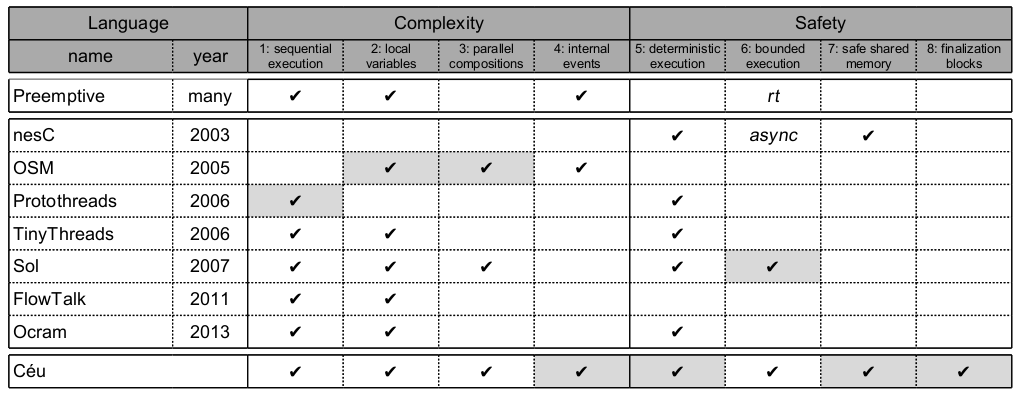
\includegraphics[width=\textwidth,clip=true,trim=110px 340px 120px 0px]{related}
\caption{ Table of features found in work related to \CEU. \newline
{\small %\textmd{
The languages are sorted by the date they first appeared in a publication.
A gray background indicates where the feature first appeared (or a contribution 
if it appears in a \CEU cell).
}%}
\label{fig.related}
}
\end{figure*}

%In this chapter we present~\ref{sec.models} we presented an overview of.

Figure~\ref{fig.related} presents an overview of work related to \CEU, pointing 
out supported features which are grouped by those that reduce complexity and 
those that increase safety.
The line \emph{Preemptive} represents asynchronous languages with preemptive 
scheduling~\cite{wsn.mantisos,wsn.tosthreads}, which are summarized further.
The remaining lines enumerate languages with goals similar to those of \CEU 
that follow a synchronous execution semantics.

Many related approaches allow events to be handled in sequence through a 
blocking primitive, overcoming the main limitation of event-driven systems 
(column~1~\cite{wsn.protothreads, wsn.ocram, wsn.tinythreads, wsn.flowtalk, 
wsn.sol}).
%
As a natural extension, most of them also keep the state of local variables 
between reactions to the environment (column~2).
In addition, \CEU introduces a reliable mechanism to interface local pointers 
with the system through finalization blocks (column~8).
%, as discussed in Section~\ref{sec.ceu.fins}.
%
Given that these approaches use cooperative scheduling, they can provide 
deterministic and reproducible execution (column~5).
%
However, as far as we know, \CEU is the first system to extend this guarantee 
for timers in parallel.

Synchronous languages first appeared in the context of WSNs through 
OSM~\cite{wsn.osm} and Sol~\cite{wsn.sol}, which provide parallel compositions 
(column~3) and distinguish themselves from multi-threaded languages by handling 
thread destruction seamlessly~\cite{sync_async.threadsstop,esterel.preemption}.
Compositions are fundamental for the simpler reasoning about control that made 
possible the safety analysis of \CEU.
%
Sol detects infinite loops at compile time to ensure that programs are 
responsive (column~6).
\CEU adopts the same policy, which first appeared in Esterel.
%
Internal events (column~4) can be used as a reactive alternative to 
shared-memory communication in synchronous languages, as supported in 
OSM~\cite{wsn.osm}.
\CEU introduces a stack-based execution that also provides a restricted but 
safer form of subroutines.
% (as discussed in Section~\ref{sec.ceu.ints}).

\emph{nesC} provides a data-race detector for interrupt handlers (column~7), 
ensuring that \emph{``if a variable x is accessed by asynchronous code, then 
any access of x outside of an atomic statement is a compile-time 
error''}~\cite{wsn.nesc}.
The analysis of \CEU is, instead, targeted at synchronous code and points more 
precisely when accesses can be concurrent, which is only possible because of 
its restricted semantics.
Furthermore, \CEU extends the analysis for system calls (\emph{commands} in 
\emph{nesC}) and control conflicts in trail termination.
Although \emph{nesC} does not enforce bounded reactions, it promotes a 
cooperative style among tasks, and provides asynchronous events that can 
preempt tasks (column 6), something that cannot be done in \CEU.
% (as discussed in Sections~\ref{sec.ceu.det} and \ref{sec.ceu.c}).

On the opposite side of concurrency models, languages with preemptive 
scheduling assume time independence among processes and are more appropriate 
for applications involving algorithmic-intensive problems.
%
Preemptive scheduling is also employed in real-time operating systems to 
provide response predictability, typically through prioritized schedulers
~\cite{wsn.mantisos,wsn.oses,freertos,wsn.tosthreads}.
%
The choice between the two models should take into account the nature of the 
application and consider the trade-off between safe synchronization and 
predictable responsiveness.
